\documentclass[../tp3_grupo404.tex]{subfiles}

\graphicspath{{\subfix{../out/}}}

\begin{document}

\subsubsection{Uso}
Para ejecutar el programa es necesario
\href{https://www.python.org/downloads/}{descargar e instalar Python 3.10}
y, desde la línea de comandos ubicado en la carpeta donde se descomprimió,
\footnote{}
ejecutar:
\begin{verbatim}
    python -m src.vuelos NOMBRE_DE_ARCHIVO
\end{verbatim}
Siendo \texttt{NOMBRE\_DE\_ARCHIVO} la ruta (relativa a la carpeta de trabajo)
al archivo con las rutas, según el formato indicado en
Formato de archivos.
Por ejemplo, para usarse con el ejemplo dado en la sección P1.1:
\begin{verbatim}
    python -m src.vuelos tests/entradas/test_ejtp3.txt
\end{verbatim}

\begin{figure}[H]
    \centering
    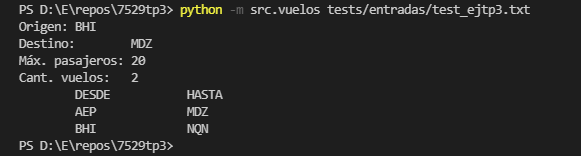
\includegraphics[width=0.9\linewidth,angle=0,origin=c]{img/captura.PNG}
    \caption{\label{screencapture}\textbf{Salida por pantalla del programa}, mismo resultado que el ejercicio.}
\end{figure}

% FIN DEL DOCUMENTO (SECCIÓN P1.4)
% NO BORRAR POR ACCIDENTE NI ESCRIBIR COSAS ABAJO
\end{document}